\documentclass[]{jarticle}          % 一段組
%\documentclass[twocolumn]{jarticle} % 二段組

\textwidth 180mm
\textheight 255mm
\oddsidemargin -12mm
\topmargin -15mm
\columnsep 10mm

%\vspace{0.5cm} % 一段組の場合はコメントアウトした方が体裁がよいx
%] % 一段組の場合はコメントアウトする

\usepackage{styles/labheadings}
\usepackage[dvipdfmx]{graphicx,color}
\usepackage{amsmath,amssymb}
\usepackage{url}
% 追加
\usepackage{listings,jvlisting}
\usepackage[hang,small,bf]{caption}
\usepackage[subrefformat=parens]{subcaption}
\captionsetup{compatibility=false}

\newcommand{\aU}{\mbox{\boldmath $a$}}
\newcommand{\bU}{\mbox{\boldmath $b$}}
\newcommand{\cU}{\mbox{\boldmath $c$}}
\newcommand{\dU}{\mbox{\boldmath $d$}}
\newcommand{\eU}{\mbox{\boldmath $e$}}
\newcommand{\fU}{\mbox{\boldmath $f$}}
\newcommand{\gU}{\mbox{\boldmath $g$}}
\newcommand{\hU}{\mbox{\boldmath $h$}}
\newcommand{\iU}{\mbox{\boldmath $i$}}
\newcommand{\jU}{\mbox{\boldmath $j$}}
\newcommand{\kU}{\mbox{\boldmath $k$}}
\newcommand{\lU}{\mbox{\boldmath $l$}}
\newcommand{\mU}{\mbox{\boldmath $m$}}
\newcommand{\nU}{\mbox{\boldmath $n$}}
\newcommand{\oU}{\mbox{\boldmath $o$}}
\newcommand{\pU}{\mbox{\boldmath $p$}}
\newcommand{\qU}{\mbox{\boldmath $q$}}
\newcommand{\rU}{\mbox{\boldmath $r$}}
\newcommand{\sU}{\mbox{\boldmath $s$}}
\newcommand{\tU}{\mbox{\boldmath $t$}}
\newcommand{\uU}{\mbox{\boldmath $u$}}
\newcommand{\vU}{\mbox{\boldmath $v$}}
\newcommand{\wU}{\mbox{\boldmath $w$}}
\newcommand{\xU}{\mbox{\boldmath $x$}}
\newcommand{\yU}{\mbox{\boldmath $y$}}
\newcommand{\zU}{\mbox{\boldmath $z$}}
\newcommand{\AU}{\mbox{\boldmath $A$}}
\newcommand{\BU}{\mbox{\boldmath $B$}}
\newcommand{\CU}{\mbox{\boldmath $C$}}
\newcommand{\DU}{\mbox{\boldmath $D$}}
\newcommand{\EU}{\mbox{\boldmath $E$}}
\newcommand{\FU}{\mbox{\boldmath $F$}}
\newcommand{\GU}{\mbox{\boldmath $G$}}
\newcommand{\HU}{\mbox{\boldmath $H$}}
\newcommand{\IU}{\mbox{\boldmath $I$}}
\newcommand{\JU}{\mbox{\boldmath $J$}}
\newcommand{\KU}{\mbox{\boldmath $K$}}
\newcommand{\LU}{\mbox{\boldmath $L$}}
\newcommand{\MU}{\mbox{\boldmath $M$}}
\newcommand{\NU}{\mbox{\boldmath $N$}}
\newcommand{\OU}{\mbox{\boldmath $O$}}
\newcommand{\PU}{\mbox{\boldmath $P$}}
\newcommand{\QU}{\mbox{\boldmath $Q$}}
\newcommand{\RU}{\mbox{\boldmath $R$}}
\newcommand{\SU}{\mbox{\boldmath $S$}}
\newcommand{\TU}{\mbox{\boldmath $T$}}
\newcommand{\UU}{\mbox{\boldmath $U$}}
\newcommand{\VU}{\mbox{\boldmath $V$}}
\newcommand{\WU}{\mbox{\boldmath $W$}}
\newcommand{\XU}{\mbox{\boldmath $X$}}
\newcommand{\YU}{\mbox{\boldmath $Y$}}
\newcommand{\ZU}{\mbox{\boldmath $Z$}}
\newcommand{\epU}{\mbox{\boldmath $\epsilon$}}
\newcommand{\taU}{\mbox{\boldmath $\tau$}}
\newcommand{\etU}{\mbox{\boldmath $\eta$}}
\newcommand{\xiU}{\mbox{\boldmath $\xi$}}
\newcommand{\wwU}{\mbox{\boldmath $\omega$}}
\newcommand{\WwU}{\mbox{\boldmath $\Omega$}}
\newcommand{\lmU}{\mbox{\boldmath $\lambda$}}
\newcommand{\LmU}{\mbox{\boldmath $\Lambda$}}
\newcommand{\PiU}{\mbox{\boldmath $\Pi$}}
\newcommand{\SgU}{\mbox{\boldmath $\Sigma$}}
\newcommand{\thU}{\mbox{\boldmath $\theta$}}
\newcommand{\ThU}{\mbox{\boldmath $\Theta$}}
\newcommand{\roU}{\mbox{\boldmath $\rho$}}
\newcommand{\nuU}{\mbox{\boldmath $\nu$}}
\newcommand{\ones}{{\bf 1}}
\newcommand{\zr}{{\bf 0}}
\newcommand{\eq}{\begin{equation}}
\newcommand{\en}{\end{equation}}
\newcommand{\eqa}{\begin{eqnarray}}
\newcommand{\ena}{\end{eqnarray}}
\newcommand{\xx}{\makebox[1cm]{}}
\newcommand{\xm}{\makebox[0.5cm]{}}
\newcommand{\x}{\makebox[0.2cm]{}}
\newcommand{\tr}{{\rm tr}}
\newcommand{\sgn}{{\rm sgn}}
\newcommand{\ad}{{\rm ad}}

\newcommand{\rank}{{\rm rank}}
\newcommand{\diag}{{\rm diag}}
\newcommand{\lbr}{\left(\begin{array}}
\newcommand{\rbr}{\end{array}\right)}
\newcommand{\Proof}{\noindent{\em Proof\/}}
\newcommand{\Solution}{\noindent{\em Solution}}
\newcommand{\Derivation}{\noindent{\em Derivation}}
\newcommand{\msp}{\vspace*{\medskipamount}\\}
\newcommand{\qed}{\hspace*{\fill}$\Box$}
\newcommand{\aX}{{\bf a}}
\newcommand{\bX}{{\bf b}}
\newcommand{\cX}{{\bf c}}
\newcommand{\dX}{{\bf d}}
\newcommand{\eX}{{\bf e}}
\newcommand{\fX}{{\bf f}}
\newcommand{\gX}{{\bf g}}
\newcommand{\hX}{{\bf h}}
\newcommand{\iX}{{\bf i}}
\newcommand{\jX}{{\bf j}}
\newcommand{\kX}{{\bf k}}
\newcommand{\lX}{{\bf l}}
\newcommand{\mX}{{\bf m}}
\newcommand{\nX}{{\bf n}}
\newcommand{\oX}{{\bf o}}
\newcommand{\pX}{{\bf p}}
\newcommand{\qX}{{\bf q}}
\newcommand{\rX}{{\bf r}}
\newcommand{\sX}{{\bf s}}
\newcommand{\tX}{{\bf t}}
\newcommand{\uX}{{\bf u}}
\newcommand{\vX}{{\bf v}}
\newcommand{\wX}{{\bf w}}
\newcommand{\xX}{{\bf x}}
\newcommand{\yX}{{\bf y}}
\newcommand{\zX}{{\bf z}}
\newcommand{\AX}{{\bf A}}
\newcommand{\BX}{{\bf B}}
\newcommand{\CX}{{\bf C}}
\newcommand{\DX}{{\bf D}}
\newcommand{\EX}{{\bf E}}
\newcommand{\FX}{{\bf F}}
\newcommand{\GX}{{\bf G}}
\newcommand{\HX}{{\bf H}}
\newcommand{\IX}{{\bf I}}
\newcommand{\JX}{{\bf J}}
\newcommand{\KX}{{\bf K}}
\newcommand{\LX}{{\bf L}}
\newcommand{\MX}{{\bf M}}
\newcommand{\NX}{{\bf N}}
\newcommand{\OX}{{\bf O}}
\newcommand{\PX}{{\bf P}}
\newcommand{\QX}{{\bf Q}}
\newcommand{\RX}{{\bf R}}
\newcommand{\SX}{{\bf S}}
\newcommand{\TX}{{\bf T}}
\newcommand{\UX}{{\bf U}}
\newcommand{\VX}{{\bf V}}
\newcommand{\WX}{{\bf W}}
\newcommand{\XX}{{\bf X}}
\newcommand{\YX}{{\bf Y}}
\newcommand{\ZX}{{\bf Z}}

% report.texと同じディレクトリにnumerical_definition.texを入れておけば上の書き方でもいいはずです

\usepackage[
  dvipdfm,
  bookmarks=true,
  bookmarksnumbered=true,
  colorlinks=true]{hyperref}
\AtBeginDvi{\special{pdf:tounicode EUC-UCS2}}

%ここからソースコードの表示に関する設定
\lstset{
  basicstyle={\ttfamily},
  identifierstyle={\small},
  commentstyle={\smallitshape},
  keywordstyle={\small\bfseries},
  ndkeywordstyle={\small},
  stringstyle={\small\ttfamily},
  frame={tb},
  breaklines=true,
  columns=[l]{fullflexible},
  numbers=left,
  xrightmargin=0zw,
  xleftmargin=3zw,
  numberstyle={\scriptsize},
  stepnumber=1,
  numbersep=1zw,
  lineskip=-0.5ex
}
%ここまでソースコードの表示に関する設定

\pagestyle{labheadings}
\headerleft{進捗報告}   % ヘッダの左側のタイトル
\headerright{2023年07月07日}  % ヘッダの右側のタイトル

\begin{document}

%\twocolumn % 一段組の場合はコメントアウトする

\vspace*{2ex}
\begin{center}
 {\Large \bf マスクの有無による特徴点の変化と三次元モデルの修正}\\ % タイトル
 \vspace*{5mm}
 {\large B4 田川幸汰}% 発表者名
\end{center}

%\vspace{0.5cm} % 一段組の場合はコメントアウトした方が体裁がよいx
%] % 一段組の場合はコメントアウトする

%新しく作成したコマンド
% \newcommand{\reffig}[1]{\hyperref[#1]{図\ref{#1}}}
% \newcommand{\refeq}[1]{\hyperref[#1]{式(\ref{#1})}}
% \newcommand{\reftab}[1]{\hyperref[#1]{表\ref{#1}}}
% \newcommand{\refsec}[1]{\hyperref[#1]{\ref{#1}章}}
% \newcommand{\refsubsec}[1]{\hyperref[#1]{\ref{#1}節}}

% 数式
%\begin{equation}
%  数式記述  
%  \label{ラベル名}
%\end{equation}

% 図
% \begin{figure}[!ht]
%   \begin{center}
%     \includegraphics[scale=0.5]{figures/画像ファイル名}
%     \caption{キャプション名}
%     \label{ラベル名}
%   \end{center}
% \end{figure}

% リスト
% \begin{enumerate or itemize}
%   \item 
% \end{enumerate or itemize}

\section{概要}
進捗報告としてZ軸方向を含めたカメラ位置推定と三次元モデル生成について発表する。 \\
また、マスク有顔画像から、マスク無顔画像を生成する研究の最終目的が、現時点でどのくらい達成できたかを報告する。

\section{Z軸方向を含めたカメラ位置、姿勢推定}
前回までの報告で、ビデオで顔の角度を変えたとき、滑らかに表示されないという問題を抱えていた。これは、
3次元座標と2次元座標からカメラ位置、姿勢を推定する際に、Z座標の値を与えていないことが原因だと推定した。
\subsection{PnP問題}
Perspectibe-n-Point問題(PnP問題)とは、世界座標系におけるn点の3次元点と
それらが画像平面へ射影された画像座標との対応から、内部パラメータが校正済みであるカメラの
外部パラメータ、つまり並進ベクトルと回転ベクトルを推定する問題のことである\cite{bib_1}。
OpenCVのSolvePnPメソッドはPnP問題を解くためのメソッドである。カメラの内部パラメータ、
3次元座標と2次元座標を引数に取り、カメラの並進ベクトルと回転ベクトルを出力する。これによってカメラの世界座標系での位置を求めることができる。
\subsection{実装}
今回は、モデルを実寸サイズに正規化したZ座標の値を含めた3次元座標と、顔の特徴点をカメラで映した2次元座標から、モデルを投影するカメラ位置を求める。
カメラ位置を求めることで、モデルを正確な大きさ、位置、角度で表示することができる。
SolvePnPメソッドには4点以上の対応する座標を与える必要がある。また、それらの座標を結んでできる四角形の面積が大きいほど、正確に対応させることができる。
今回はマスクで隠れない位置で、かつ面積が大きな四角形が作れるように、mediapipeで取得した67番、297番、145番、374番の特徴点を与えた。
Mediapipeで取得した特徴点の位置を\hyperref[one]{図\ref{one}}に示す。
\begin{figure}[!ht]
  \begin{center}
    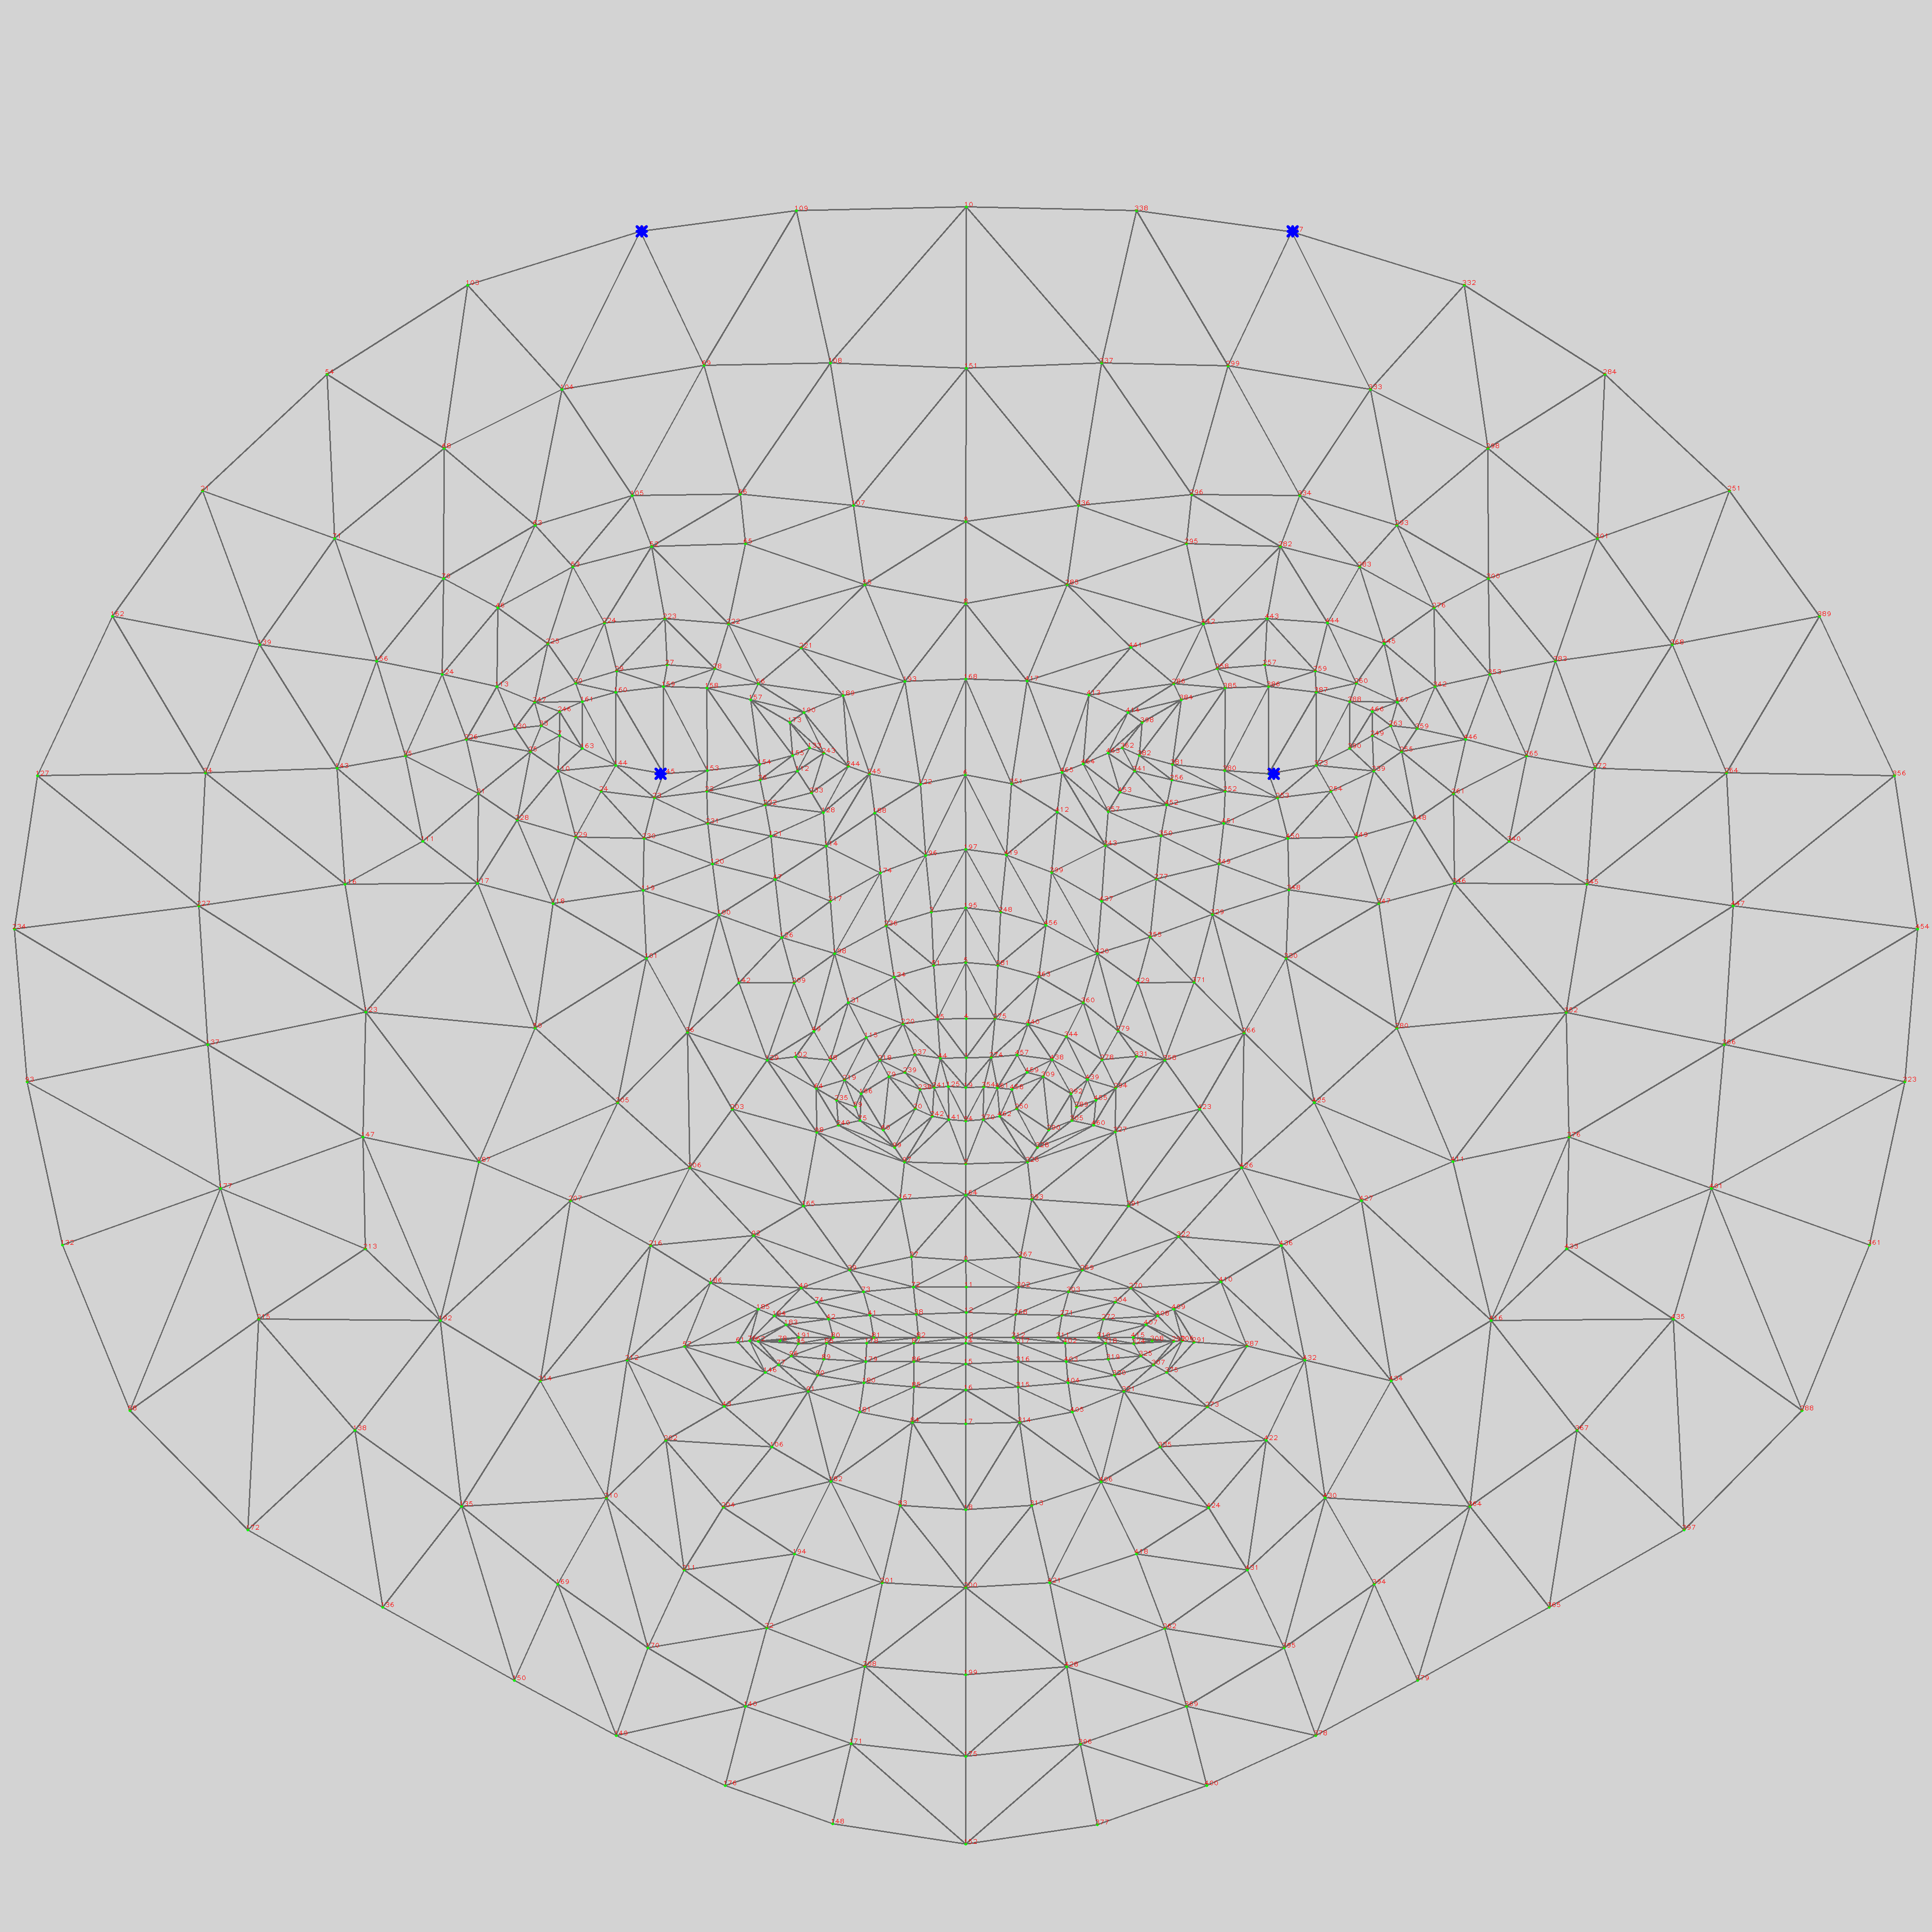
\includegraphics[scale=0.07]{figures/test.png}
    \caption{facemeshの特徴点}
    \label{one}
  \end{center}
\end{figure}

\newpage

\subsection{実行結果}
プログラムを実行した結果、顔の角度を上下左右に変えても滑らかに表示された。
また、対応する座標の位置を変えたことによる影響は、マスクを着けていない場合は特になかった。
実行中の画像を\hyperref[two]{図\ref{two}}、\hyperref[three]{図\ref{three}}に示す。
\begin{figure}[!ht]
  \begin{tabular}{cc}
    \begin{minipage}[t]{0.45\hsize}
      \centering
      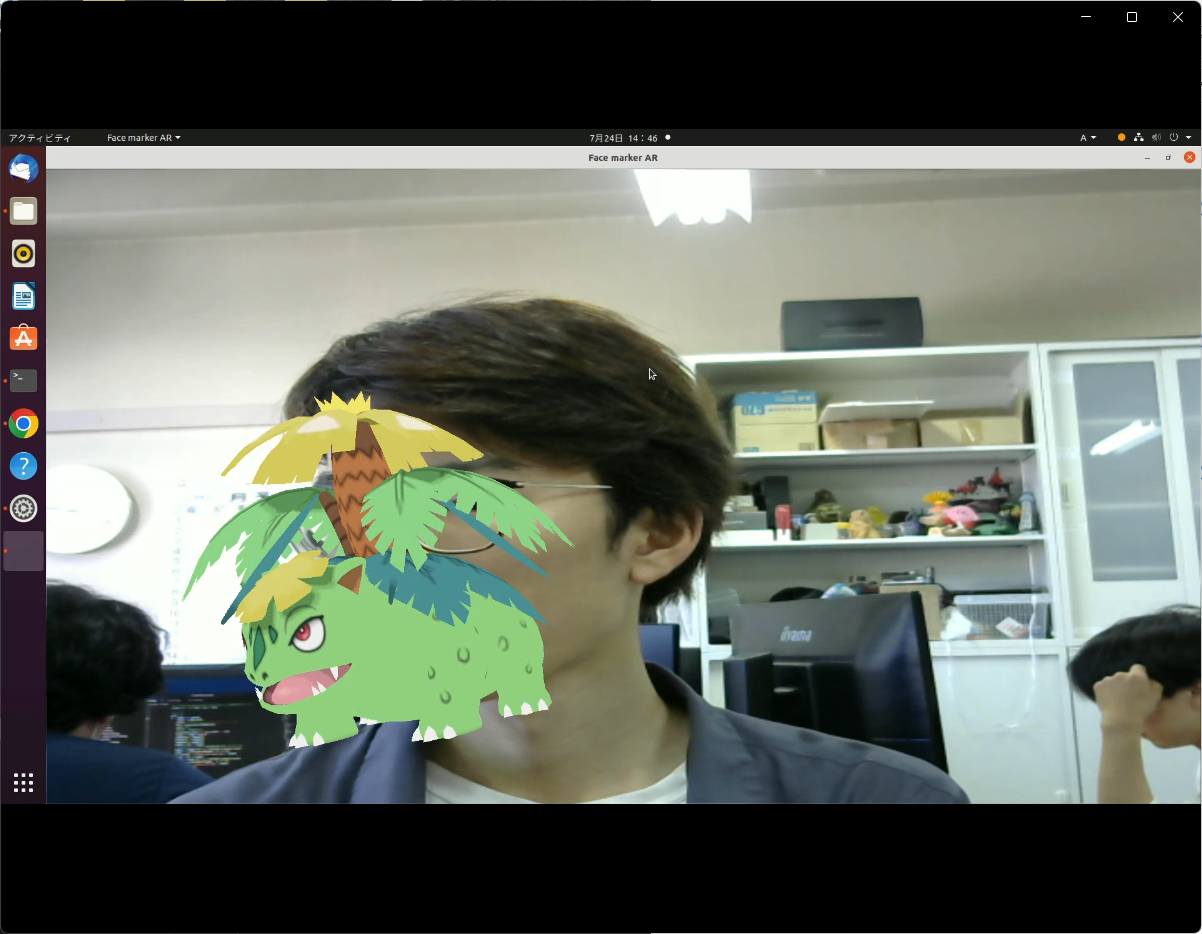
\includegraphics[keepaspectratio, scale=0.2]{figures/output1.png}
      \caption{Z軸を含む正規化後の実行画像}
      \label{two}
    \end{minipage} &
    \begin{minipage}[t]{0.45\hsize}
      \centering
      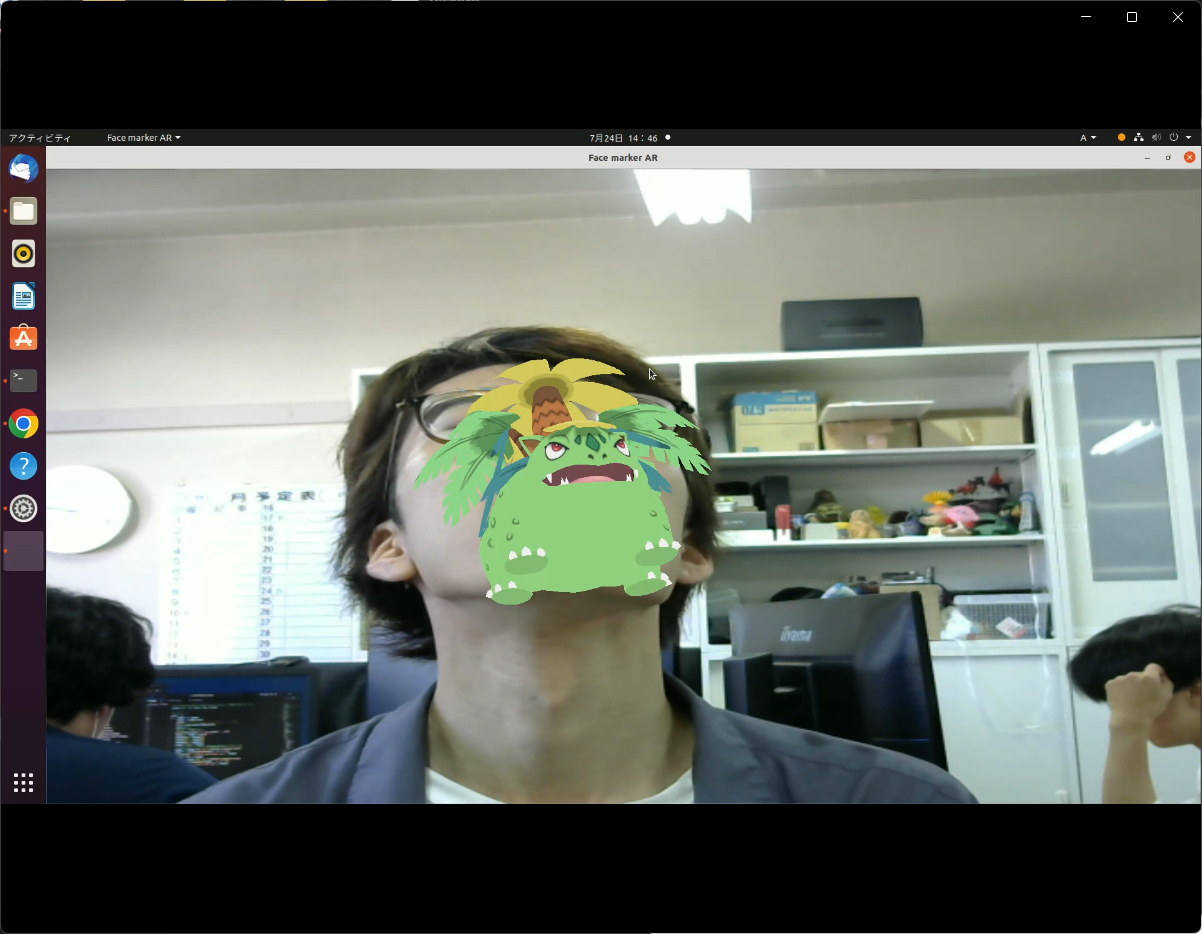
\includegraphics[keepaspectratio, scale=0.2]{figures/output2.png}
      \caption{Z軸を含む正規化後の実行画像}
      \label{three}
    \end{minipage}
  \end{tabular}
\end{figure}

\newpage

\section{三次元モデルの生成}
テクスチャ画像を入力することで三次元モデルを作成するプログラムを資料\cite{bib_2}を参考にしながら作成した。また、作成した三次元モデルは
これまでに作成した、顔モデルを顔の特徴点に合わせて貼り付けるプログラムに渡され、そのまま実行できるように調整した。

\subsection{実装}
任意のテクスチャ画像からfacemeshと同じ頂点数を持つ三次元モデルを生成するプログラムを、以下の手順で作成した。
\begin{enumerate}
  \item テクスチャ画像を入力から読み込む。
  \item 三角形メッシュの特徴点情報のファイルを読み込む。
  \item mediapipeのfacemeshにより、テクスチャ画像の特徴点の三次元座標を求める。
  \item テクスチャ画像の特徴点の三次元座標を、実際の座標系に合うように変換した三次元座標を求める。
  \item テクスチャ画像と特徴点情報のファイル、3、4で求めた三次元座標を基に、三次元モデルを作成する。
\end{enumerate}
3で求めた特徴点の三次元座標は、$X,Y,Z$軸方向がそれぞれ$[0:1],[0:1],[-1:1]$の範囲で正規化されたものとする。
ここで、4で行った三次元座標の座標系変換について次の節で詳しく述べる。
\subsection{三次元座標変換}
座標系変換を以下の手順で行った。
\begin{enumerate}
  \item 特徴点の座標のアスペクト比を修正する \\
        テクスチャ画像のサイズが$W\times{H}$であるとき、\hyperref[four]{式\ref{four}}のように特徴点座標を変換する。
        \begin{equation}
          (X,Y,Z){\leftarrow}(X\times{W},Y\times{H},Z\times{W})
          \label{four}
        \end{equation}
  \item 基準とする位置が三次元座標の原点となるように平行移動する \\
        今回は、基準とする座標(つまり、世界座標系の原点となる座標の位置)を鼻先の点(ランドマークID:1)の座標$P_{base}$とする。
        この場合、\hyperref[five]{式\ref{five}}のようにすべての点を平行移動する。
        \begin{equation}
          P_a^{\prime}{\leftarrow}P_a-P_{base}
          \label{five}
        \end{equation}        
  \item 実際の大きさにスケーリングする \\
        今回は実際の顔の大きさになる基準として、左右の目の端の間の長さ$(100mm)$とした。座標大きさの基準となる2点間の距離がそれぞれ、実際の距離では$L$, ランドマーク間の距離では$l$であると
        き, \hyperref[six]{式\ref{six}}のようにすべての点をスケーリングする。
        \begin{equation}
          P_a^{\prime\prime}{\leftarrow}\frac{L}{l}P_a^{\prime}
          \label{six}
        \end{equation}                
\end{enumerate}
また、これまではモデルの表示部分でモデルのスケールや位置を変更していたが、座標系変換を行うことで、その必要がなくなった。

\subsection{実行結果}
入力したテクスチャ画像を\hyperref[seven]{図\ref{seven}}に示す。
また、これにより作成された三次元モデルを\hyperref[eight]{図\ref{eight}}に示す。
\begin{figure}[!ht]
  \begin{tabular}{cc}
    \begin{minipage}[t]{0.45\hsize}
      \centering
      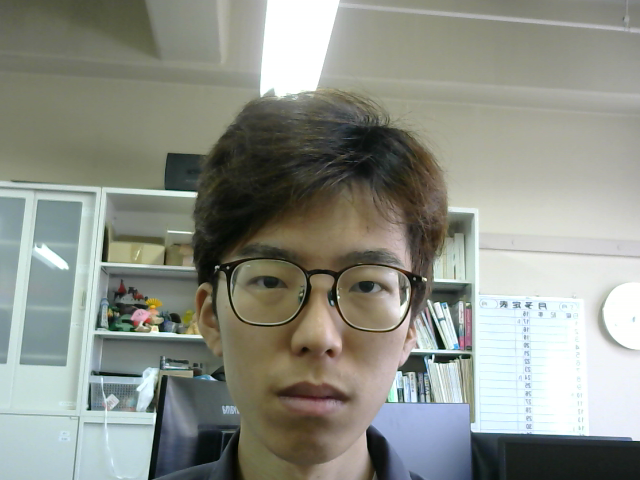
\includegraphics[keepaspectratio, scale=0.2]{figures/texture.png}
      \caption{テクスチャ画像}
      \label{seven}
    \end{minipage} &
    \begin{minipage}[t]{0.45\hsize}
      \centering
      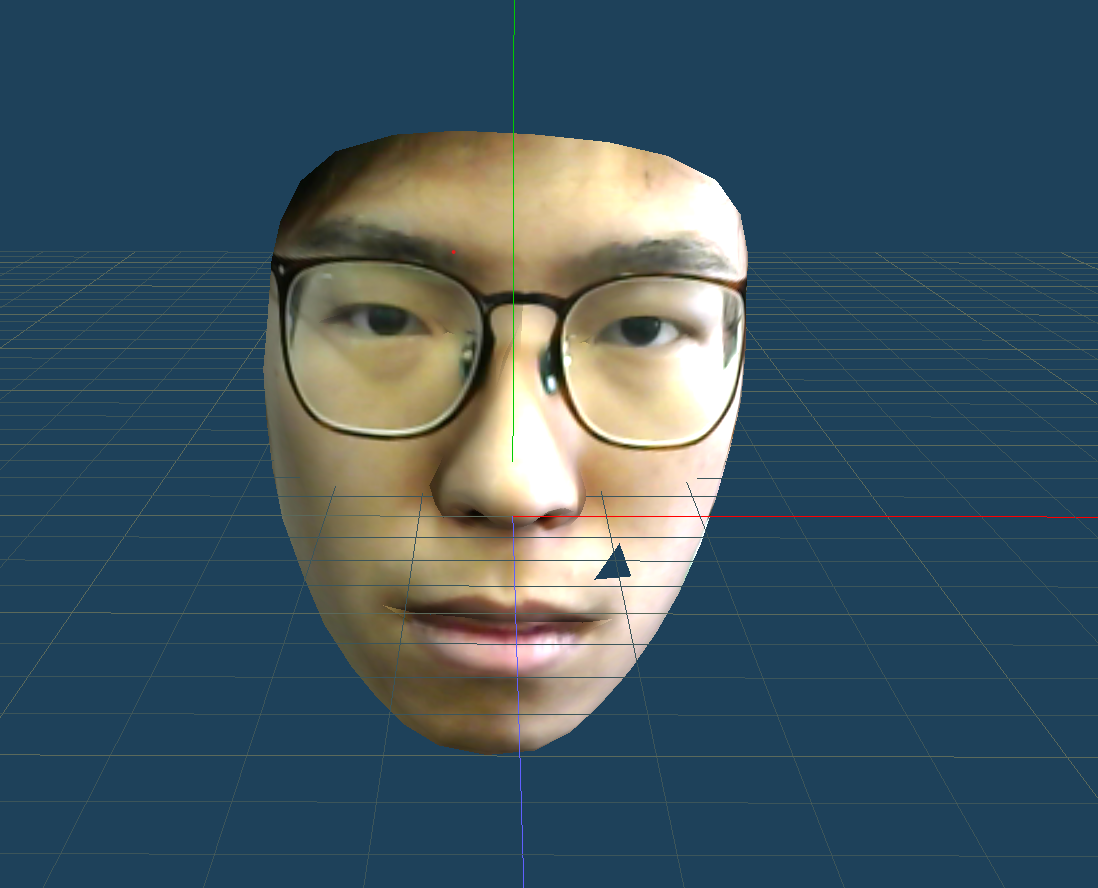
\includegraphics[keepaspectratio, scale=0.2]{figures/3dmodel.png}
      \caption{三次元モデル}
      \label{eight}
    \end{minipage}
  \end{tabular}
\end{figure}

\newpage

また、これにより作成された三次元モデルを、顔の特徴点に合わせて貼り付けた結果を\hyperref[nine]{図\ref{nine}}、
\hyperref[ten]{図\ref{ten}}に示す。
\begin{figure}[!ht]
  \begin{tabular}{cc}
    \begin{minipage}[t]{0.45\hsize}
      \centering
      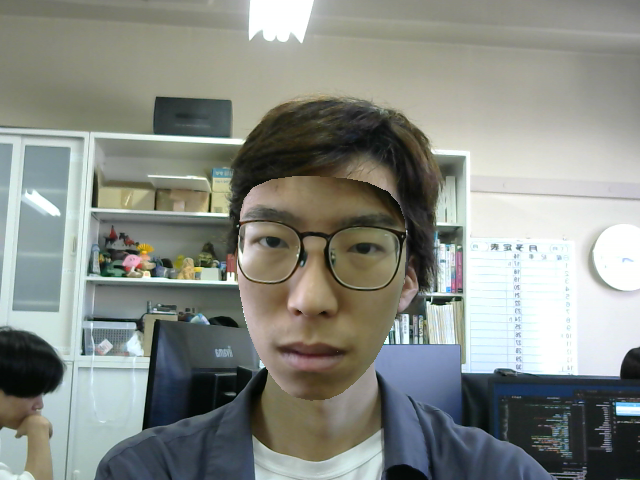
\includegraphics[keepaspectratio, scale=0.3]{figures/output3.png}
      \caption{実行結果(マスクなし)}
      \label{nine}
    \end{minipage} &
    \begin{minipage}[t]{0.45\hsize}
      \centering
      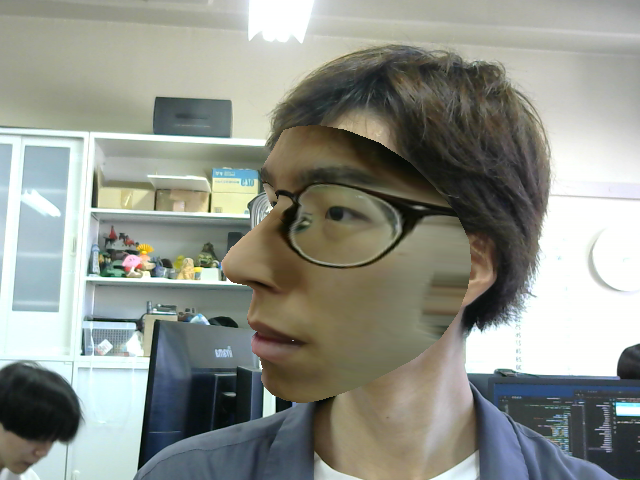
\includegraphics[keepaspectratio, scale=0.3]{figures/output4.png}
      \caption{実行結果(マスクなし)}
      \label{ten}
    \end{minipage}
  \end{tabular}
\end{figure}
この結果から、マスクなしの場合テクスチャ画像から三次元モデルを作成し、実際に検出された顔の特徴点に合わせて貼り付けることができた。
モデルに髪の毛が映り込んだり、少し倍率があっていないような部分もあるので、そのあたりも適宜修正していきたい。

\section{マスク有顔画像スク無顔画像を生成}
先ほどまでの章ではマスクなしの状態で顔三次元モデルを貼り付けた結果について報告した。
以降はマスクありの状態で顔三次元モデルを貼り付けた場合、どのような結果が得られたか発表する。
\subsection{実行結果}
入力したテクスチャ画像及び作成した三次元モデルは先ほどと同じである。
三次元モデルを、マスクありの顔の特徴点に合わせて貼り付けた結果を\hyperref[eleven]{図\ref{eleven}}、
\hyperref[twelve]{図\ref{twelve}}に示す。
\begin{figure}[!ht]
  \begin{tabular}{cc}
    \begin{minipage}[t]{0.45\hsize}
      \centering
      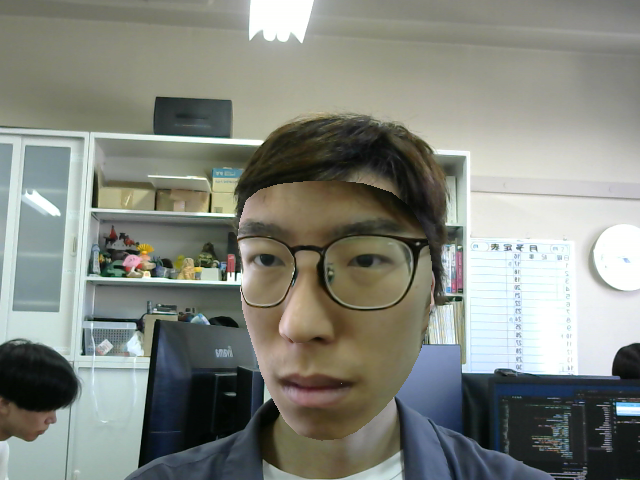
\includegraphics[keepaspectratio, scale=0.3]{figures/output5.png}
      \caption{実行結果(マスクあり)}
      \label{eleven}
    \end{minipage} &
    \begin{minipage}[t]{0.45\hsize}
      \centering
      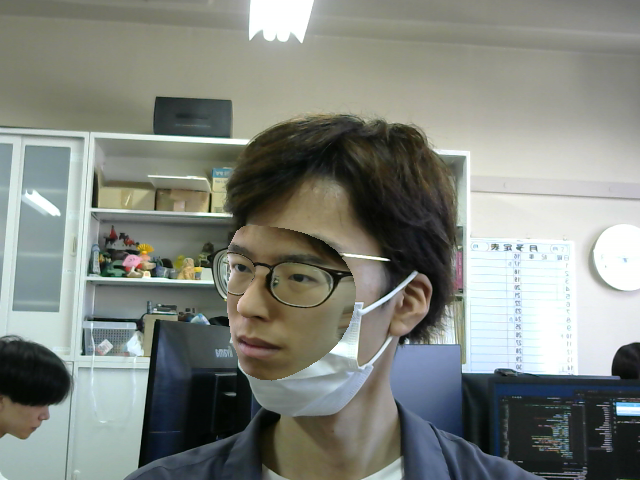
\includegraphics[keepaspectratio, scale=0.3]{figures/output6.png}
      \caption{実行結果(マスクあり)}
      \label{twelve}
    \end{minipage}
  \end{tabular}
\end{figure}
この結果から、顔が正面の角度の場合は、マスクありの場合とほぼ同じように表示することができている。
しかし顔に角度がある場合は、正しくモデルを貼り付けることができていない。
また、顔の特徴点を検出するmediapipeのfacemeshが実行できているか調べたところ、角度をつけた場合は
実行できていないことがわかった。つまり、マスクをつけている部分、つけていない部分に限らずすべての座標が検出できていないことになる。\\

\section{研究計画}
現時点で進行中の研究や、次回の発表時までに進めたい研究計画を以下にまとめる。\\
\\
進行中
\begin{itemize}
  \item 顔上の特徴点を用いた類似研究の論文の査読
  \item mediapipe iris (虹彩検出)を利用した推定
\end{itemize}

%参考文献
\begin{thebibliography}{99}
\bibitem{bib_1} 中野学,Perspectibe-n-Point問題とその派生問題に対する安定かつ高速な解放に関する研究,閲覧日2023/7/26
\bibitem{bib_2} 菅谷保之,FaceMeshを利用した実寸サイズの3次元顔モデルの作成,閲覧日2023/7/26
\end{thebibliography}

\end{document}
